\chapter{}

\section{Screen Shot}

\begin{figure}[H]\centering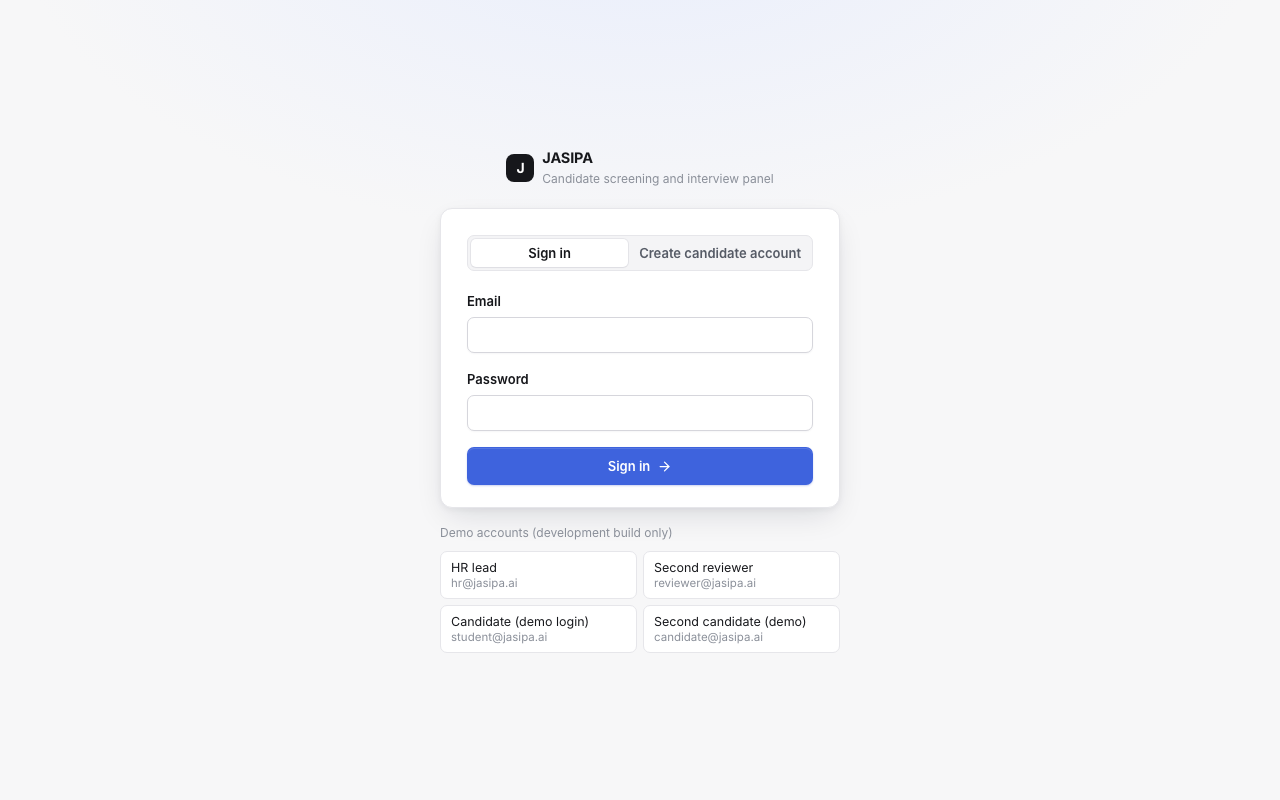
\includegraphics[width=0.85\textwidth]{../screenshots/01-login.png}
\caption{Sign-in page}\label{fig:ss-login}\end{figure}

\begin{figure}[H]\centering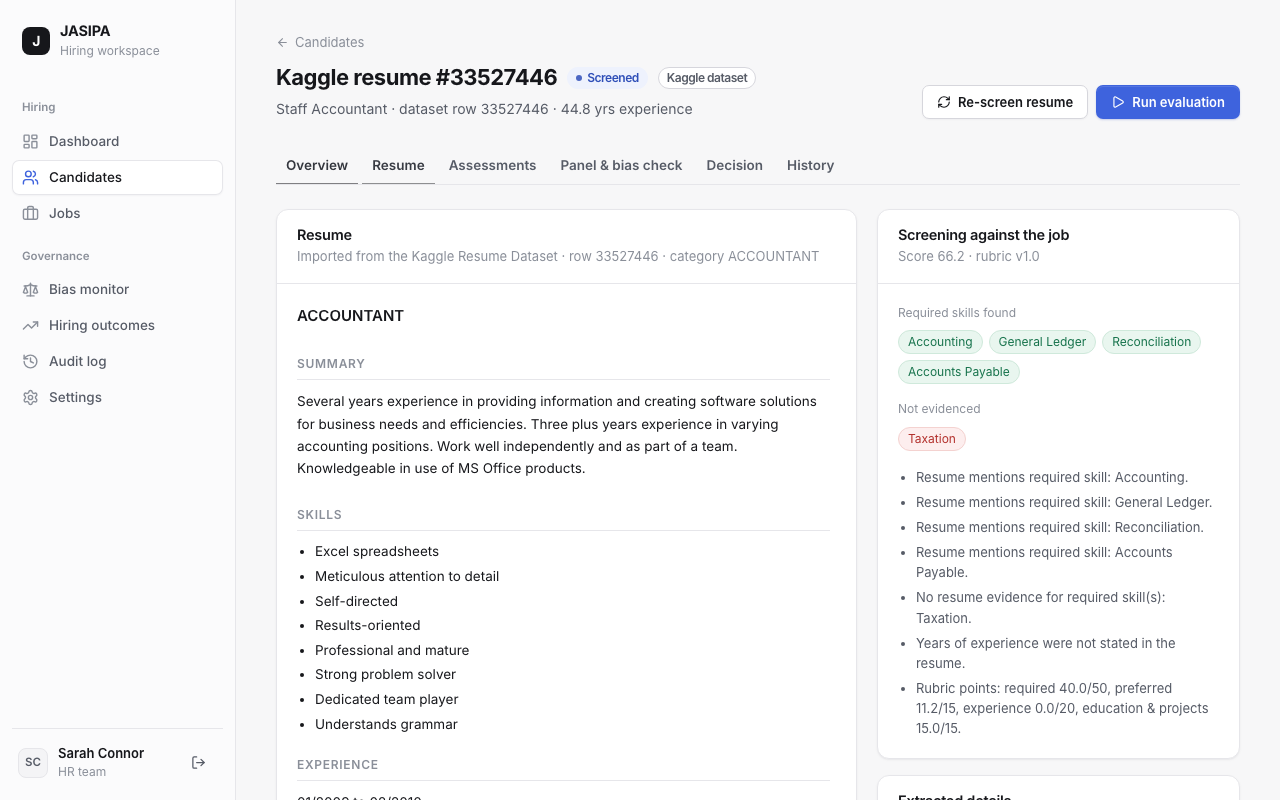
\includegraphics[width=0.85\textwidth]{../screenshots/09-dataset-resume.png}
\caption{Kaggle dataset record displayed in its original sections}\label{fig:ss-dataset}\end{figure}

\begin{figure}[H]\centering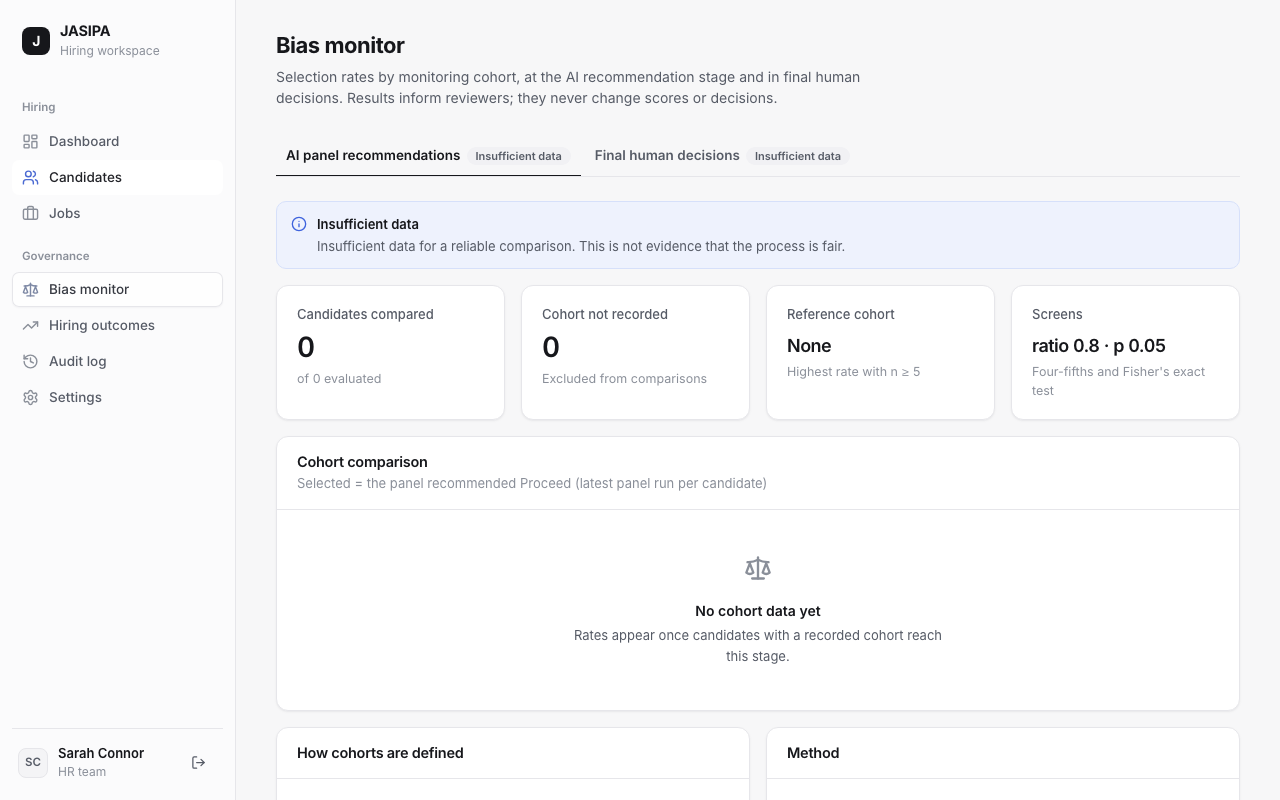
\includegraphics[width=0.85\textwidth]{../screenshots/10-bias-monitor.png}
\caption{Bias monitor showing the cohort definition, method and missing-cohort count}\label{fig:ss-monitor}\end{figure}

\begin{figure}[H]\centering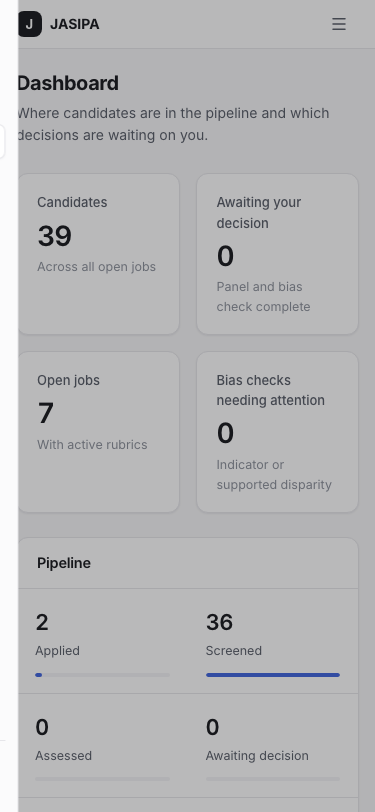
\includegraphics[height=0.45\textheight]{../screenshots/11-mobile.png}
\caption{Responsive layout at 375$\times$812}\label{fig:ss-mobile}\end{figure}

\section {Gantt Chart}
\begin{figure}[H]\centering\resizebox{\textwidth}{!}{% Built from the repository commit history (git log); dates are commit dates.
\begin{tikzpicture}[x=5mm, y=-7mm]
\foreach \d/\l in {0/18 Sep, 5/23 Sep, 10/28 Sep, 15/3 Oct, 20/8 Oct, 23/11 Oct} {\node[lbl] at (\d+0.5,-0.2) {\l}; \draw[draw=line] (\d,0.2) -- (\d,8.6);}
\newcommand{\gbar}[4]{\fill[#4, rounded corners=1pt] (#1,#3-0.32) rectangle (#2,#3+0.32);}
\node[lbl, anchor=east] at (-0.3,1) {Initial system build};
\node[lbl, anchor=east] at (-0.3,2) {Candidate portal, auth, UI clean-up};
\node[lbl, anchor=east] at (-0.3,3) {Secrets hygiene};
\node[lbl, anchor=east] at (-0.3,4) {Fallback strategies, fairness checks};
\node[lbl, anchor=east] at (-0.3,5) {Rubric balancing, audit ledger, governance};
\node[lbl, anchor=east] at (-0.3,6) {Backend rework: agents, sandbox, bias, upload};
\node[lbl, anchor=east] at (-0.3,7) {Frontend redesign and removals};
\node[lbl, anchor=east] at (-0.3,8) {Kaggle data, regeneration fix, tests, docs};
\gbar{0}{11}{1}{accent!55} \gbar{11}{12}{2}{accent!55} \gbar{12}{13}{3}{accent!55} \gbar{13}{17}{4}{accent!55}
\gbar{17}{21}{5}{accent!55} \gbar{23}{24}{6}{green!70} \gbar{23}{24}{7}{green!70} \gbar{23}{24}{8}{green!70}
\end{tikzpicture}
}
\caption{Project schedule}\label{fig:gantt}\end{figure}

\section {Glossary}
\begin{description}
\item[ATS] Applicant tracking system: the database of jobs, candidates and applications.
\item[Cohort] An HR-recorded monitoring label used only for fairness statistics.
\item[Four-fifths rule] Adverse-impact screen: a cohort's selection rate below 80\% of the highest cohort's rate.
\item[Impact ratio] A cohort's selection rate divided by the reference cohort's rate.
\item[Fisher's exact test] Exact significance test for a 2$\times$2 table of selected/not selected by cohort.
\item[Wilson interval] Confidence interval for a proportion, reliable for small $n$.
\item[MCP] Model Context Protocol: a JSON-RPC protocol through which agents call external tools.
\item[STAR] Situation, Task, Action, Result: a structure for behavioural answers.
\item[Rubric] Versioned scoring criteria and weights derived from a job description.
\item[Swarm] Several agents working in parallel on separate evidence, merged by a coordinator.
\item[JWT] JSON Web Token used for authenticated API sessions.
\end{description}

\section {Description of Tools and  Technology used}
\begin{table}[H]\centering\small\caption{Tools and technologies}
\begin{tabular}{|p{3.6cm}|p{10.4cm}|}\hline
\textbf{Tool} & \textbf{Use}\\ \hline
Python 3.12, FastAPI & REST API, dependency-injected authentication and RBAC\\ \hline
SQLAlchemy 2, SQLite/PostgreSQL & ORM and storage with additive migrations\\ \hline
LangGraph & Agent state graph with parallel evaluator branches\\ \hline
Google Gemini (optional) & LLM strategies for scoring, question drafting and summaries\\ \hline
PyMuPDF, python-docx & Resume text extraction\\ \hline
bcrypt, python-jose & Password hashing and JWT\\ \hline
React 19, Vite 8 & Single-page frontend\\ \hline
pytest, Vitest, Testing Library, Playwright & Automated tests\\ \hline
Docker (optional) & Hardened code-execution backend\\ \hline
\LaTeX\ (Tectonic), TikZ & Report and diagrams\\ \hline
Git, GitHub & Version control\\ \hline
\end{tabular}\end{table}

\section{Blue Print}

Attach your Blue Print file at the end

\section{Plagiarism Report}

Attach your Plagiarism Report file at the end
